\specialchap{序言}

随着物理学的发展,人们对于世界的理解也越来越深入。在粒子物理相关的研究中,组成世界的基本粒子一共有12种,分为6种夸克,3种带电轻子以及3种中微子。随着对于这十二种粒子的深入研究和理解,人们在量子场论的框架下基于量子色动力学和弱电相互统一理论,构建了标准模型(Standard Model, SM)。标准模型成功解释了宇宙中物质的构成以及它们之间的相互作用,并被大量的实验所证实。2012年标准模型所预测的最后一种粒子——希格斯玻色子被发现,更是完美地符合了标准模型的预测。

在标准模型所描述的基本粒子中,中微子显得十分地神秘和特殊。对中微子的研究最早可以追溯到1930年,奥地利物理学家泡利(Wolfgang Ernst Pauli)在一封解释$\beta$衰变能谱连续问题的信中,首次提出$\beta$衰变可能会产生一种微小的电中性粒子。随后这个假设被费米(Enrico Fermi)引入到了他的$\beta$衰变理论中\supercite{wilson1968fermi}。1956年,随着Clyde Cowan和Frederick Reines在实验中首次确认了电子中微子的存在\supercite{cowan1991detection},人们才开始了解这一神秘的基本粒子。$\mu$中微子于1962年被Brookhaven国家实验室所发现\supercite{danby1962observation},而后直到2000年,最后一种中微子$\tau$中微子存在的直接证据才被费米实验室找到\supercite{kodama2001observation}。

在标准模型中中微子被认为是没有质量的,但是大量过去和进行中的中微子实验,如超级神冈(Super-Kamiokande)\supercite{fukuda1998evidence},萨德伯里中微子观测站(SNO)\supercite{ahmad2002direct}等,都观测到了中微子震荡现象。在对于该现象的诸多解释中,最为自然的是中微子并非如标准模型所预言的质量为零,而是拥有一个极小的质量。这一理论可能标志着在标准模型之外,未被探索的新物理的存在。

中微子既然可能拥有质量,它质量的来源便是一个十分有趣的问题。如果假设中微子是狄拉克费米子(Dirac fermions),那么为了使它产生微小的质量,中微子与希格斯场相互作用的耦合系数会比夸克等其他粒子小12个量级,如此巨大的差别令人难以信服。另一种假设是中微子是马约拉纳费米子(Majorana fermions),即它自身是自己的反粒子,相对而言这种模型更为自洽,但它也意味着标准模型中轻子数守恒的推断将会被打破,也将为理论物理带来巨大的改变。然而到现在为止,还没有足够的实验观测能够判断哪种模型更为正确。

在中微子到底是何种费米子的相关研究中,有一类实验致力于寻找被称作无中微子双Beta衰变(Neutrinoless double beta decay, NLDBD)\supercite{avignone2008double}的稀有事件。在标准模型中,有一些核素因为束缚能的原因不能发生单次Beta衰变,但是它们可以通过一个次级的弱相互作用来同时释放出两个电子(正电子)和两个反中微子(中微子),如图\ref{fig:nldbd}(a)所示,这种衰变模式被称作双Beta衰变(Double beta decay, DBD)。双Beta衰变事件虽然稀有但它已经被实验所观测和证实。如果中微子是马约拉纳费米子,即中微子和反中微子是同一种粒子,那么双Beta衰变中第一次释放出的反中微子(中微子)又可能作为中微子(反中微子)参与第二次衰变。对外体现为核素直接衰变出两个电子(正电子)而不产生反中微子(中微子),如图\ref{fig:nldbd}(b)所示。这种现象就被称作无中微子双Beta衰变事件。

\begin{figure}
    \centering
    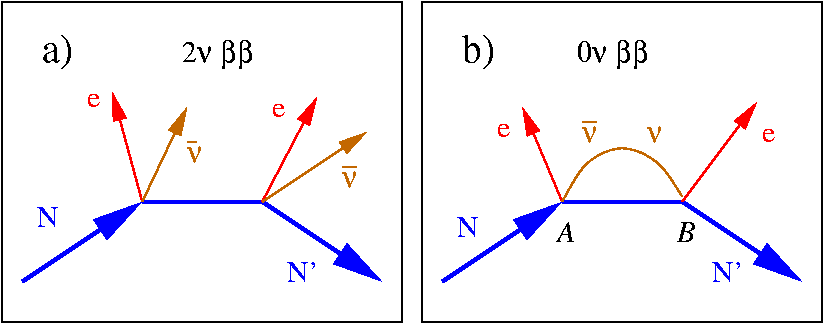
\includegraphics[width=0.5\columnwidth]{pic/nldbd.png}
    \caption{有中微子双Beta衰变(a)以及无中微子双Beta衰变(b)示意图。}
    \label{fig:nldbd}
\end{figure}

如果NLDBD事件被证实,那么不但意味着轻子数不再守恒,中微子的质量也可以通过其半衰期计算得到,如公式\ref{eq1}所示\supercite{avignone2008double},其中$G^{0\nu}$是相空间因子,$M^{0\nu}$是核矩阵元素。从公式中可以看出,如果NLDBD事件的半衰期$T^{0\nu}_{1/2}$已知,那么可以通过公式求得马约拉纳中微子质量$\langle m_{\beta\beta}\rangle$。中微子绝对质量量级和中微子的质量顺序也可以由$\langle m_{\beta\beta}\rangle$进一步计算得到,从而加深人们对于中微子的认识和了解。

\begin{equation}
    (T_{1/2}^{0\nu})^{-1}=G^{0\nu}|M^{0\nu}|^2\frac{\langle m_{\beta\beta}\rangle ^2}{m_e^2}
    \label{eq1}
\end{equation}

近年来世界上很多实验组都在进行NLDBD事件的探测,根据2015年美国核科学顾问局的报告\supercite{NLDBD_NSAC},现在正在进行的实验有CUORE\supercite{Artusa:2014lgv}, EXO-200\supercite{Albert:2014awa}, GERDA\supercite{Agostini:2016iid}, KamLAND-Zen\supercite{KamLAND-Zen:2016pfg}, Majorana\supercite{Abgrall:2013rze},SNO+\supercite{Andringa:2015tza}等。目前最好的实验结果是KamLAND-Zen给出的$^{136}$Xe NLDBD事件的半衰期$T^{0\nu}_{1/2}>1.07\times10^{26}$年。在经过广泛的交流后,这些NLDBD实验组们达成了普遍的共识:至少需要1吨量级的放射性同位素才有可能通过探测NLDBD事件来确定中微子的质量顺序。为了顺利的达成这一实验目的,不仅仅需要能够顺利的生产出吨量级的放射性同位素,同时需要极佳的探测器分辨率和极低的本底噪声,以及鉴别NLDBD
和本底的方法。

粒子和天气物理氙探测器第三期实验(Particle And Astrophysical Xenon Experiment III,以下简称PandaXIII)便是一个设计中的吨级的$^{136}$Xe无中微子双Beta衰变探测实验,它使用高压气氙时间漂移室(TPC)作为探测器,放置于锦屏地下实验室来屏蔽宇宙射线本底,并计划在两到三年内建立出第一个200kg级探测器。本文详细描述了PandaXIII实验设计和前期测试中模拟的相关工作,分为以下几个部分。第一章将会简单介绍整个项目,第二章描述了探测器模拟中本底模拟的相关工作,第三章介绍了如何使用卷积神经网络(Convolution Neural Network, CNN)来鉴别本底事件和信号,第四章给出了原型探测器测试标定过程中的模拟工作。上述工作是本文作者主要参与的,PandaXIII项目中探测器设计,电子学等其他相关工作的描述可以参见PandaXIII中期设计报告\supercite{cdr}。

% vim:ts=4:sw=4